%==============================================================================
%vvvvvvvvvvvvvvvvvvvvvvvvvvvvvvvvvvvvvvvvvvvvvvvvvvvvvvvvvvvvvvvvvvvvvvvvvvvvvv

\documentclass{beamer}
\usepackage[utf8]{inputenc}
\usepackage[ngerman]{babel} % neue deutsche Rechtschreibung 
\usepackage{babelbib}       % deutsches Literaturverzeichnis
\usepackage{verbatim} 



% Background
\usepackage{tikz}
\usetikzlibrary{fadings}
\setbeamertemplate{background}{
\begin{tikzpicture}
\path (0,0) rectangle (\paperwidth,\paperheight);
\node[scope fading=west,inner sep=0pt,outer sep=0pt,anchor=north east] at(\paperwidth*1.3,\paperheight*0.83) {
\includegraphics[height=\paperheight]{pics/uni}};
\end{tikzpicture}
}

\PassOptionsToPackage{usenames}{color} 
\usepackage{color} 
\usepackage[usenames]{color} 


%^^^^^^^^^^^^^^^^^^^^^^^^^^^^^^^^^^^^^^^^^^^^^^^^^^^^^^^^^^^^^^^^^^^^^^^^^^^^^^
%==============================================================================
%vvvvvvvvvvvvvvvvvvvvvvvvvvvvvvvvvvvvvvvvvvvvvvvvvvvvvvvvvvvvvvvvvvvvvvvvvvvvvv

\usetheme{default}
\usecolortheme{seagull}
% Remove navigation
\beamertemplatenavigationsymbolsempty
% \setcounter{tocdepth}{2}
\usecaptiontemplate{
  \tiny
  \insertcaption
}


% Use bullet as item for lists
\setbeamertemplate{itemize items}{$\bullet$}

% %\setbeamertemplate{itemize subitem}{{\tiny $\spadesuit$}}
% %\setbeamertemplate{itemize subsubitem}{{\tiny $\heartsuit$}}
% \setbeamertemplate{footline}[frame number]
% \setbeamertemplate{sections/subsections in toc}[circle]{}

%^^^^^^^^^^^^^^^^^^^^^^^^^^^^^^^^^^^^^^^^^^^^^^^^^^^^^^^^^^^^^^^^^^^^^^^^^^^^^^
%==============================================================================




\title{Per-Circuit TCP-over-IPsec Transport\\for Anonymous Communication Overlay Networks}   
\author{Manuel Schneider}
\institute{Albert Ludwigs Universität - Institut für Informatik} 
\date{\today} 

%==============================================================================
%//////////////////////////////////////////////////////////////////////////////
%//////////////////////////////////////////////////////////////////////////////
%//////////////////////////////////////////////////////////////////////////////
\begin{document}%//////////////////////////////////////////////////////////////
%//////////////////////////////////////////////////////////////////////////////
%//////////////////////////////////////////////////////////////////////////////
%//////////////////////////////////////////////////////////////////////////////
%==============================================================================

\begin{frame}
  \titlepage
\end{frame}


\begin{frame}{Motivation}
gfsdfs
\end{frame}

%==============================================================================
%//////////////////////////////////////////////////////////////////////////////
\section{TOR}
%//////////////////////////////////////////////////////////////////////////////
%==============================================================================



\begin{frame}{\textsc{Tor} - Architektur/Terminologie}
  \begin{figure}
    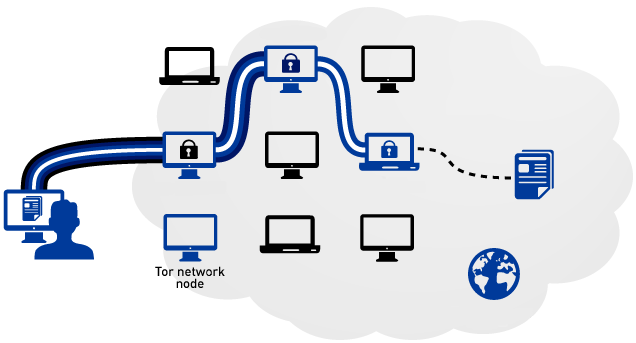
\includegraphics[width=\textwidth]{pics/tor}
  \end{figure}
Das Große und Ganze
Onion Routing, Cell, Circuit, Stream, Onion Router,- Proxy
\end{frame}



\begin{frame}{Cells - Das \textsc{Tor} Tranportmittel}
 
  \begin{columns}[c]
  
    \column{.45\textwidth}
    \begin{figure}
      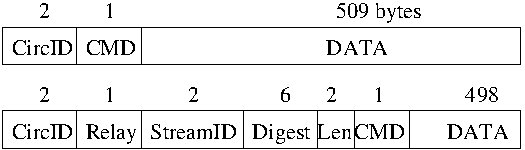
\includegraphics[width=\textwidth]{pics/cell}
      \caption{Quelle: \cite{tor}}
    \end{figure}
    
    \column{.55\textwidth}
    \begin{block}{Control Cell}
      \begin{itemize}
	\item Dienen dem Management der Circuits
	\begin{itemize}
	  \item Aufbau, Abbau, Keepalive
	\end{itemize}
	\item Werden vom Onion Router interpretiert, der sie empfängt
      \end{itemize}
    \end{block} 
    \begin{block}{Relay Cell}
      \begin{itemize}
	\item Zur Weiterleitung der Daten auf dem Circuit
	\item Zusätzlicher Relay Header
      \end{itemize}
    \end{block} 
  
    \begin{itemize}
      \item Beide haben Circuit Identifier
    \end{itemize}
    
  \end{columns}
\end{frame}

\begin{frame}{Circuits - Die \textsc{Tor} Transportwege}
  \begin{figure}
    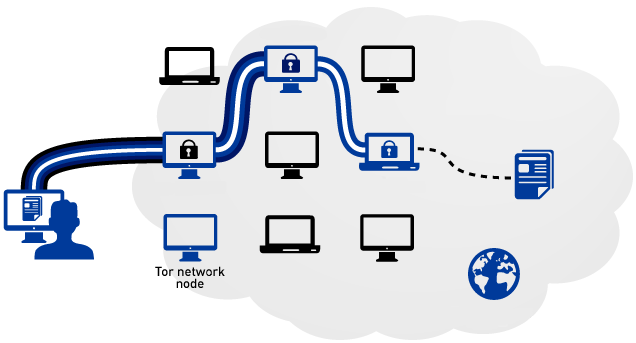
\includegraphics[width=.6\textwidth]{pics/tor}
  \end{figure}
  \begin{itemize}
    \item Pfade im Netzwerk entlang welcher die Cells gesendet werden
    \item Werden Hop-by-hop aufgebaut
    \begin{itemize}
      \item Mit jedem Knoten wird ein Schlüssel ausgehandelt
    \end{itemize}
    \item Üblicherweise drei: Entry\-, Middle-, Exit Node
    \item Jeder Hop hat einen Circuit Identifier
    \item Werden nach einem Zeitintervall oder Fehler gewechselt
    \item Werden auf Vorrat angelegt (Performace)
  \end{itemize}
\end{frame}

 
\begin{frame}{Circuits - Inkrementeller Aufbau}

  \only<1>
  {
    \begin{itemize}
      \item OP holt Informationen beim Directory Server 
      \begin{itemize}
	\item Router descriptor: Public Keys, Bandbreite, Adresse der OR
      \end{itemize}      
      \item Onion Proxy wählt anhand Exit Policies eine Exit Node
      \item Danach weitere Onion Router,\\ sodass jeder nur einmal vorkommt
    \end{itemize}
  }
  
  \only<2>
  {
    \begin{itemize}
      \item \textcolor{brown}{Create} Control Cell an OR\,1
	\begin{itemize}
	  \item Enthält Diffie-Hellman Handshake
	  \item OR\,1 kennt nun den Schlüssel
	  \item Circuit Identifier wurde von Alice festgelegt
	\end{itemize}
      \item \textcolor{brown}{Created} Control Cell zurück (OP kennt nun den Schlüssel)
	\begin{itemize}
	  \item Alice kennt nun den Schlüssel
	\end{itemize}
    \end{itemize}
    \begin{figure}
    \centering{
      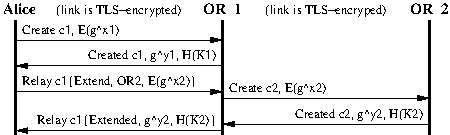
\includegraphics[width=0.8\textwidth]{pics/extension}
      \caption{Quelle: \cite{tor}}}
    \end{figure}
  }
\end{frame}


\begin{frame}{Cross Circuit Interference Problem.}
  \begin{figure}
    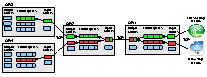
\includegraphics[width=0.8\textwidth]{pics/BufferPic.pdf}
    \caption{ Quelle: \cite{pctcp}}
  \end{figure} 
\end{frame}


\begin{frame}{Head On Line Blocking}
  \begin{figure}
    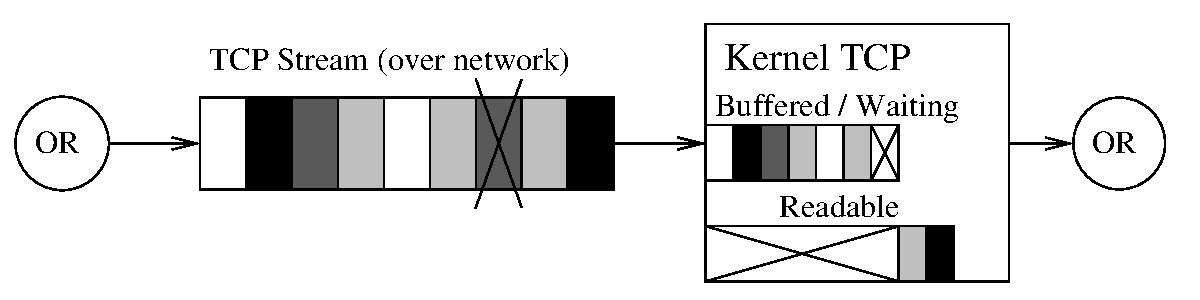
\includegraphics[width=0.7\textwidth]{pics/headonlinevanilla.pdf}
    \caption{Quelle: \cite{tcp-over-dtls}}
  \end{figure}
\end{frame}


%==============================================================================
%//////////////////////////////////////////////////////////////////////////////
\section{IPSec}
%//////////////////////////////////////////////////////////////////////////////
%==============================================================================

\begin{frame}{Internet Protocol Security (IPSec)}
  \begin{itemize}
    \item Arbeitet auf Vermittlungsschicht
    \item Stellt Schutzziele sicher
    \begin{itemize}
      \item Vertraulichkeit
      \item Authentizität
      \item Integrität
    \end{itemize}
    \item Umfasst Protkolle für eine gesicherte Kommunikation
    \begin{itemize}
      \item Authentication Header (AH)
      \item Encapsulating Security Payload (ESP)
    \end{itemize}
    \item Je zwei Betriebsmodi
    \begin{itemize}
      \item Transport Modus
      \item Tunnel Modus
    \end{itemize}
  \end{itemize}
\end{frame}


\begin{frame}{IPSec - Protokolle}
 \begin{block}{IP Authentication Header (AH)}
  \begin{itemize}
   \item Stellt Authentizität und Integrität der Daten sicher
   \item Authentifiziert Sender 
   \item Schützt gegen Replay-Angriffe
   \item Inkompatibel mit Network Adress Translation!
  \end{itemize}
 \end{block}
 \begin{block}{IP Encapsulating Security Payload (ESP)}
  \begin{itemize}
   \item Selbes Featureset wie AH
   \item Stellt zusätzlich Vertraulichkeit der Daten sicher
  \end{itemize}
 \end{block}
\end{frame}


\begin{frame}{IPSec - Betriebsmodi}
  \begin{figure}
    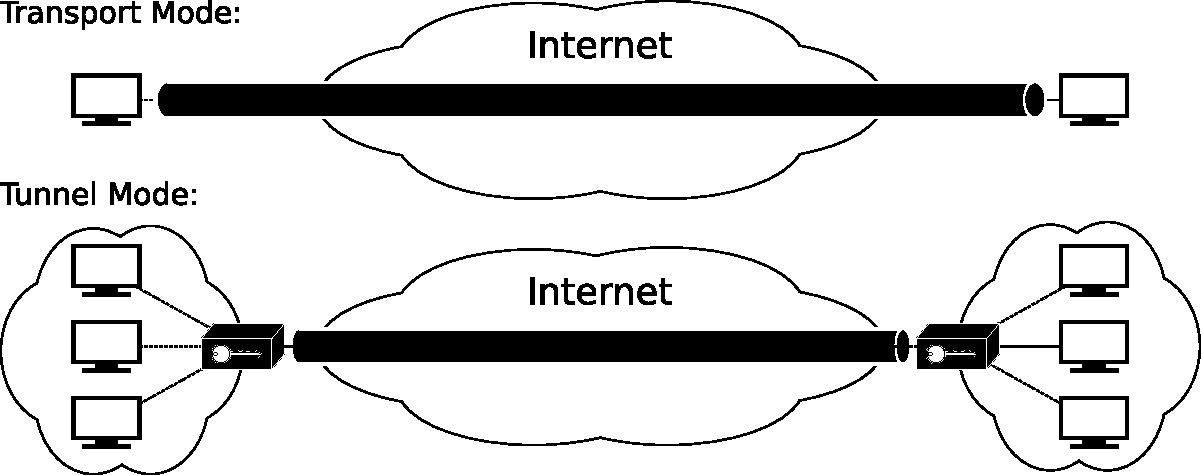
\includegraphics[width=0.7\textwidth]{pics/modes}
    \caption{Quelle: www.wikimedia.com}
  \end{figure} 
  \only<1>
  {
    \begin{block}{Transport Modus}
      \begin{itemize}
	\item IP Header bleibt unberührt, auch bei ESP
      \end{itemize}
    \end{block} 
  }
  \only<2>
  {
    \begin{block}{Tunnel Modus}
      \begin{itemize}
	\item Zusätzlicher IP Header 
      \end{itemize}
    \end{block} 
  }
\end{frame}

%==============================================================================
%//////////////////////////////////////////////////////////////////////////////
\section{PCTCP}
%//////////////////////////////////////////////////////////////////////////////
%==============================================================================


\begin{frame}{PCTCP Design}
  \begin{figure}
    \begin{center}
      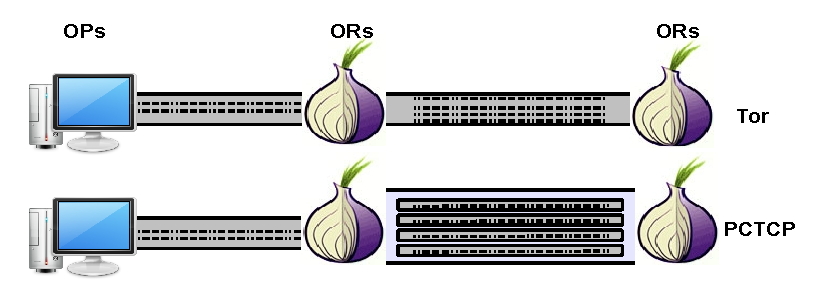
\includegraphics[width=0.7\textwidth]{pics/PCTCP_design.pdf}
      \caption{Vergleich des Designs zwischen Standard-\textsc{Tor} und PCTCP.}
    \end{center}
  \end{figure} 
\end{frame}


\begin{frame}{IPSec in PCTCP}
  \begin{figure}[h]
  \centering{
    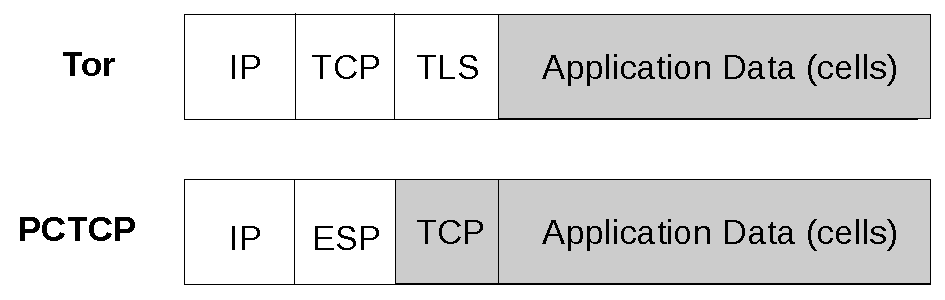
\includegraphics[width=0.7\textwidth]{pics/PCTCP_header.pdf}
    \caption{Vergleich der Inter Onion Router Pakete zwischen Standard-\textsc{Tor} und PCTCP.Grau schattierte Teile sind verschlüsselt. Quelle:\cite{pctcp}}}
  \end{figure} 
\end{frame}


\begin{frame}{PCTCP - Ciruit construction}
\end{frame}




%==============================================================================
%//////////////////////////////////////////////////////////////////////////////
\section{Diskussion}
%//////////////////////////////////////////////////////////////////////////////
%==============================================================================

\begin{frame}{Ease of deployment}
\end{frame}

\begin{frame}{Socket Exhaustion Attacks}
\end{frame}

\begin{frame}{Ausblick}
Kurz sagen, dass PCTCP beinahe genauso wenig taugt wie TCPoverDTLS und warum.
Vielleicht IMUX anreisen
\end{frame}



%===============================================================================
%///////////////////////////////////////////////////////////////////////////////
%///////////////////////////////////////////////////////////////////////////////
%///////////////////////////////////////////////////////////////////////////////
%===============================================================================

\begin{frame}[plain]{Reference}
  \begin{center}
  Vielen Dank für die Aufmerksamkeit!
  \end{center}
  \tiny
  \bibliographystyle{plain}
  \bibliography{bibliography}
\end{frame}

\nocite{tor}
\nocite{tcp-over-dtls}
\nocite{pctcp}
\nocite{imux}
\nocite{tor_improvements}

%===============================================================================
%///////////////////////////////////////////////////////////////////////////////
%///////////////////////////////////////////////////////////////////////////////
%///////////////////////////////////////////////////////////////////////////////
%///////////////////////////////////////////////////////////////////////////////
\end{document}%/////////////////////////////////////////////////////////////////
%///////////////////////////////////////////////////////////////////////////////
%///////////////////////////////////////////////////////////////////////////////
%///////////////////////////////////////////////////////////////////////////////
%///////////////////////////////////////////////////////////////////////////////
%==============================================/=================================
